% ============================================================
%  FactorBoosting – Technical Presentation
%  Beamer · Metropolis theme (169 aspect ratio)
%  Covers: Portfolio Construction, Weighting, TC, Metrics, IR
% ============================================================
\documentclass[aspectratio=169, 12pt]{beamer}

% ── Theme ────────────────────────────────────────────────────
\usetheme{metropolis}
\usepackage{appendixnumberbeamer}

% ── Packages ─────────────────────────────────────────────────
\usepackage{amsmath, amssymb}
\usepackage{booktabs}
\usepackage{xcolor}
\usepackage{listings}
\usepackage{hyperref}
\usepackage{tikz}
\usepackage{pgfplots}
\pgfplotsset{compat=1.18}
\usetikzlibrary{arrows.meta, positioning, shapes.geometric}

% ── Colour palette ───────────────────────────────────────────
\definecolor{primary}{HTML}{3B4CCA}
\definecolor{accent}{HTML}{10B981}
\definecolor{warning}{HTML}{F59E0B}
\definecolor{danger}{HTML}{EF4444}
\definecolor{codebg}{HTML}{1E1E2E}
\definecolor{codehl}{HTML}{3B82F6}
\definecolor{lightgray}{HTML}{F4F4F5}

\setbeamercolor{frametitle}{bg=primary, fg=white}
\setbeamercolor{progress bar}{fg=accent}
\setbeamercolor{alerted text}{fg=accent}

% ── Code listing style ───────────────────────────────────────
\lstdefinestyle{jscode}{
  backgroundcolor=\color{codebg},
  basicstyle=\ttfamily\tiny\color{white},
  keywordstyle=\color{codehl}\bfseries,
  commentstyle=\color{gray}\itshape,
  stringstyle=\color{accent},
  numberstyle=\tiny\color{gray},
  numbers=left,
  numbersep=5pt,
  breaklines=true,
  showstringspaces=false,
  frame=none,
  tabsize=2,
  morekeywords={const,let,function,return,if,else,for,of,new,true,false,null,
                Math,Number,Set,Map,async,await},
}

% ── Metadata ─────────────────────────────────────────────────
\title{FactorBoosting -- Technical Methodology}
\subtitle{Portfolio Construction, Transaction Costs \& Performance Analytics}
\author{Safexpress Centre for Data, Learning and Decision Sciences\\
        Ashoka University}
\date{2026}

% ============================================================
\begin{document}
% ============================================================

\maketitle

\begin{frame}{Agenda}
  \tableofcontents[hideallsubsections]
\end{frame}

% ============================================================
\section{Platform Overview}
% ============================================================

\begin{frame}{What is FactorBoosting?}
  \begin{columns}[T]
    \begin{column}{0.55\textwidth}
      \textbf{An open, interactive backtesting platform} for Indian equity factor research.
      \medskip
      \begin{itemize}
        \item \textbf{Data:} Oct 2003 -- May 2026
        \item \textbf{Universe:} Top 300 / Top 500 NSE stocks
        \item \textbf{Rebalancing:} Monthly
        \item \textbf{Comparison:} Up to 5 simultaneous portfolios
        \item \textbf{TC sensitivity:} Live transaction-cost sweep
        \item \textbf{Benchmarks:} NIFTY 50 \& NIFTY 500
      \end{itemize}
    \end{column}
    \begin{column}{0.4\textwidth}
      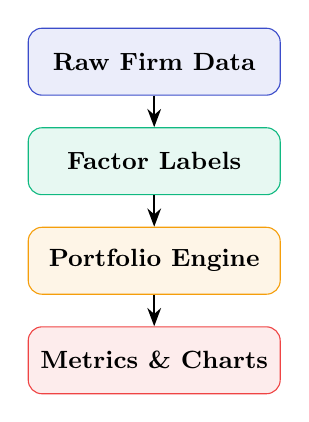
\begin{tikzpicture}
        \node[draw=primary, fill=primary!10, rounded corners=5pt,
              minimum width=3.2cm, minimum height=0.85cm,
              font=\small\bfseries] (data) {Raw Firm Data};
        \node[draw=accent, fill=accent!10, rounded corners=5pt,
              minimum width=3.2cm, minimum height=0.85cm,
              font=\small\bfseries, below=0.4cm of data] (label) {Factor Labels};
        \node[draw=warning, fill=warning!10, rounded corners=5pt,
              minimum width=3.2cm, minimum height=0.85cm,
              font=\small\bfseries, below=0.4cm of label] (port) {Portfolio Engine};
        \node[draw=danger, fill=danger!10, rounded corners=5pt,
              minimum width=3.2cm, minimum height=0.85cm,
              font=\small\bfseries, below=0.4cm of port] (metrics) {Metrics \& Charts};
        \draw[-{Stealth}, thick] (data) -- (label);
        \draw[-{Stealth}, thick] (label) -- (port);
        \draw[-{Stealth}, thick] (port) -- (metrics);
      \end{tikzpicture}
    \end{column}
  \end{columns}
\end{frame}

% ============================================================
\section{Factor Universe \& Data}
% ============================================================

\begin{frame}{The 10 Factors Available}
  \begin{columns}[T]
    \begin{column}{0.48\textwidth}
      {\color{primary}\textbf{Classic Factors (FF5 + Momentum)}}
      \smallskip
      \begin{tabular}{ll}
        \toprule
        Factor & Labels \\
        \midrule
        Size & Big (B), Small (S) \\
        Book-to-Market & G, Neutral, Value \\
        Profitability & Robust, N, Weak \\
        Investment & Agg., N, Conserv. \\
        Momentum & Winner, N, Loser \\
        \bottomrule
      \end{tabular}
    \end{column}
    \begin{column}{0.48\textwidth}
      {\color{accent}\textbf{Other Factors}}
      \smallskip
      \begin{tabular}{ll}
        \toprule
        Factor & Labels \\
        \midrule
        Asset Turnover & H, Neutral, L \\
        Sales Growth & H, Neutral, L \\
        Accruals & Cons., N, Agg. \\
        Volatility & Low, N, High \\
        Short-Term Rev. & Loser, N, Winner \\
        \bottomrule
      \end{tabular}
    \end{column}
  \end{columns}
  \vspace{4pt}
  \begin{alertblock}{Size Label Selection}
    \textbf{Monthly} size labels: Momentum, Volatility, Short-Term Reversal.\\
    \textbf{Annual} size labels: BM, Investment, Profitability, and all other factors.
  \end{alertblock}
\end{frame}

\begin{frame}{Data Sources \& Return Sanitization}
  \begin{itemize}
    \item \textbf{Factor panel:} PostgreSQL (Supabase) + cached JSON snapshots for fast access
    \item \textbf{Benchmarks:} NIFTY 50 \& NIFTY 500 monthly returns from \texttt{benchmark\_monthly}
    \item \textbf{Risk-free rate:} 91-day T-Bill monthly rate from \texttt{ff5.csv} (\texttt{Rf} column)
  \end{itemize}
  \medskip
  \textbf{Return Sanitization Pipeline:}
  \begin{enumerate}
    \item \textbf{Drop} if $r = \mathrm{NaN}$ or $r \notin \mathbb{R}$
    \item \textbf{Drop} if $r \leq r_{\min}$ or $r \geq r_{\max}$ (configurable bounds; currently $\pm\infty$)
    \item \textbf{Winsorize} if $r > \text{cap}_{\mathrm{hi}}$ or $r < \text{cap}_{\mathrm{lo}}$ (preserves direction)
    \item Otherwise \textbf{accept} row
  \end{enumerate}
  Zeroing outliers biases returns downward; winsorisation at the cap value is therefore preferred.
\end{frame}

% ============================================================
\section{Portfolio Construction}
% ============================================================

\begin{frame}{Monthly Construction Pipeline}
  For each month $t$ in the backtest window:

  \medskip
  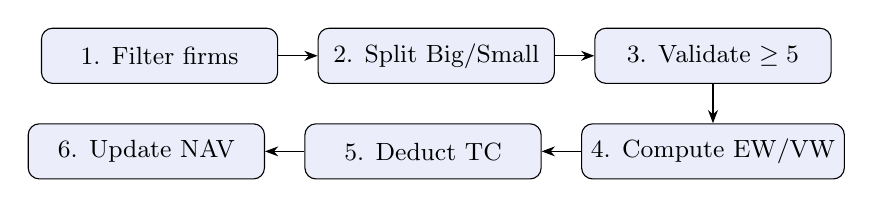
\begin{tikzpicture}[node distance=0.5cm, font=\small,
      box/.style={draw, rounded corners=4pt, fill=primary!10,
                  minimum width=3.0cm, minimum height=0.7cm, align=center}]
    \node[box] (f)  {1. Filter firms};
    \node[box, right=0.5cm of f]  (s)  {2. Split Big/Small};
    \node[box, right=0.5cm of s]  (v)  {3. Validate $\geq5$};
    \node[box, below=0.5cm of v]  (w)  {4. Compute EW/VW};
    \node[box, left=0.5cm of w]   (tc) {5. Deduct TC};
    \node[box, left=0.5cm of tc]  (c)  {6. Update NAV};
    \draw[-{Stealth}] (f)--(s); \draw[-{Stealth}] (s)--(v);
    \draw[-{Stealth}] (v)--(w); \draw[-{Stealth}] (w)--(tc);
    \draw[-{Stealth}] (tc)--(c);
  \end{tikzpicture}

  \vspace{6pt}
  \textbf{Minimum-firm rule:} A size-factor cell is only included if it contains
  $\geq 5$ firms with valid monthly returns.

  For long-short: if \emph{either} leg has $< 5$ firms in a given size bucket,
  \textbf{both sides of that size bucket} are dropped for that month.
\end{frame}

\begin{frame}{Equal-Weighted (EW) Return}
  For a set of $N$ firms with valid returns $\{r_{i,t}\}$:
  \[
    R_t^{\text{EW}} = \frac{1}{N} \sum_{i=1}^{N} r_{i,t}
  \]

  When \emph{both} Small and Big size buckets are valid:
  \[
    R_t^{\text{EW}} = \frac{R_t^{\text{EW,Small}} + R_t^{\text{EW,Big}}}{2}
  \]
  (macro equal-weight across size groups; within each group, firms are equally weighted)

  \medskip
  \textbf{Long-short:}
  \[
    R_t^{\text{EW,LS}} = R_t^{\text{EW,Long}} - R_t^{\text{EW,Short}}
  \]
\end{frame}

\begin{frame}{Value-Weighted (VW) Return}
  Each firm $i$ is weighted by its \textbf{lagged} market capitalisation $m_{i,t-1}$:
  \[
    R_t^{\text{VW}} = \frac{\displaystyle\sum_{i=1}^{N} m_{i,t-1}\, r_{i,t}}{\displaystyle\sum_{i=1}^{N} m_{i,t-1}}
  \]
  \begin{itemize}
    \item Firms with missing $m_{i,t-1}$ fall back to equal-weighting within their cell
    \item When both size buckets are valid:
    \[
      R_t^{\text{VW}} = \frac{R_t^{\text{VW,Small}} + R_t^{\text{VW,Big}}}{2}
    \]
    (equal macro-weight between size groups; within each, VW by market cap)
  \end{itemize}

  \begin{alertblock}{Pure-Size L/S: BM Neutralisation}
    For a pure Size factor portfolio (e.g.\ Long Big, Short Small), the engine averages
    across three BM terciles (G, N, V) that each satisfy the $\geq5$ firm minimum,
    removing incidental Value exposure.
  \end{alertblock}
\end{frame}

\begin{frame}{Cumulative NAV}
  Portfolio starts at an index of 100 and compounds monthly:
  \[
    V_t = V_{t-1} \cdot (1 + R_t^{\text{net}})
  \]
  where $R_t^{\text{net}}$ is the portfolio return \emph{after} transaction costs.

  \medskip
  Returns are capped to $[-200\%,\;+200\%]$ before compounding (data sanity guard to prevent NAV explosion from extreme single observations).
\end{frame}

% ============================================================
\section{Transaction Cost Model}
% ============================================================

\begin{frame}{Transaction Cost: Motivation}
  Real-world factor strategies incur costs at every rebalance event:
  \begin{itemize}
    \item \textbf{Brokerage / commissions} -- explicit per-trade cost
    \item \textbf{Bid-ask spread} -- implicit market-impact cost
    \item \textbf{Slippage} -- execution price vs.\ quoted price
  \end{itemize}

  \medskip
  Ignoring transaction costs systematically \textbf{overstates} net-of-trading returns,
  especially for high-turnover factors such as \textit{Momentum} and \textit{Short-Term Reversal}.

  \medskip
  \begin{alertblock}{Our approach}
    A single \textbf{one-way basis-points} parameter multiplied by the portfolio's
    weight-drift-adjusted monthly turnover.
  \end{alertblock}
\end{frame}

\begin{frame}{Turnover: Weight-Drift Adjustment}
  After month $t-1$, weights drift with individual stock returns.
  The \textbf{drift-adjusted} weight of firm $i$ entering month $t$ is:
  \[
    \tilde{w}_{i,t-1} = \frac{w_{i,t-1}^{\vphantom{EW}} \cdot (1 + r_{i,t-1})}{1 + R_{t-1}^{\text{gross}}}
  \]
  This properly reflects what the portfolio actually holds \emph{before} rebalancing,
  without needing to assume a reset to target weights at zero cost.

  \medskip
  Applied separately to EW and VW weight maps.
\end{frame}

\begin{frame}{Turnover Calculation}
  Monthly turnover for EW (and analogously for VW):
  \[
    \tau_t^{\text{EW}} = \sum_{i \in \mathcal{U}_t} \bigl|w_{i,t}^{\text{EW}} - \tilde{w}_{i,t-1}^{\text{EW}}\bigr|
  \]
  where $\mathcal{U}_t = \{\text{firms in current or prior portfolio}\}$.

  \medskip
  This naturally captures:
  \begin{itemize}
    \item \textbf{New entries} -- stock $i$ not in prior portfolio: $\tilde{w}_{i,t-1} = 0$
    \item \textbf{Full exits} -- stock $i$ not in current portfolio: $w_{i,t} = 0$
    \item \textbf{Partial rebalances} -- weight change within a continuing holding
  \end{itemize}

  Average monthly turnover reported:
  \[
    \bar{\tau} = \frac{1}{T}\sum_{t=1}^{T} \frac{\tau_t^{\text{EW}} + \tau_t^{\text{VW}}}{2} \times 100\%
  \]
\end{frame}

\begin{frame}{From Basis Points to Net Return}
  \textbf{User input:} $c$ basis points (bps).

  \medskip
  \textbf{Conversion to decimal fraction:}
  \[
    \text{cost fraction} = \frac{c}{10{,}000}
  \]

  \textbf{Net monthly return:}
  \[
    R_t^{\text{EW,net}} = R_t^{\text{EW,gross}} - \tau_t^{\text{EW}} \cdot \frac{c}{10{,}000}
  \]

  \medskip
  \begin{columns}[T]
    \begin{column}{0.48\textwidth}
      \textbf{Interpretation of ``one-way'':}\\
      $c = 10$ bps means each unit of weight traded costs 10 bps.\\
      A full round-trip (enter then exit) costs $2c = 20$ bps.
    \end{column}
    \begin{column}{0.48\textwidth}
      \textbf{Formation month:}\\
      By default, TC is \emph{not} applied to the very first portfolio formation (month index $= 0$).\\
      Optionally enabled via \texttt{includeFormation}.
    \end{column}
  \end{columns}
\end{frame}

\begin{frame}[fragile]{Implementation: Parsing the TC Input}
\begin{lstlisting}[style=jscode]
// backtest-engine.js -- lines 528-536
function normalizeTransactionCost(input = {}) {
  // If mode is not "bps", return a zero-cost passthrough
  if (input.mode !== "bps")
    return { mode: "none", cost: 0, includeFormation: false };

  const bps = Number.parseFloat(input.bps ?? input.costBps ?? 0);

  return {
    mode: "bps",
    cost: Number.isFinite(bps) ? bps / 10000 : 0,  // convert bps -> fraction
    includeFormation: Boolean(input.includeFormation),
  };
}
\end{lstlisting}
\end{frame}

\begin{frame}[fragile]{Implementation: Drift-Adjusted Weight Update}
\begin{lstlisting}[style=jscode]
// backtest-engine.js -- lines 782-788
// After computing this month's gross return, update prev weights for next month.
// Weights drift with individual stock returns; normalise by portfolio gross return.
const ewDenom = 1 + (ewGross || 0);
const vwDenom = 1 + (vwGross || 0);

for (const [code, w] of currWeights.entries()) {
  // w.r = this firm's monthly return; w.ew / w.vw = current portfolio weight
  if (ewDenom > 0) prevEwWeights.set(code, (w.ew * (1 + w.r)) / ewDenom);
  if (vwDenom > 0) prevVwWeights.set(code, (w.vw * (1 + w.r)) / vwDenom);
}
// prevXxWeights is carried into the next month's turnover calculation
\end{lstlisting}
\end{frame}

\begin{frame}[fragile]{Implementation: Turnover \& Cost Deduction}
\begin{lstlisting}[style=jscode]
// backtest-engine.js -- lines 758-778
let monthEwTurnover = 0, monthVwTurnover = 0;
// Union of all stocks in current AND previous portfolio
const allCodes = new Set([...prevEwWeights.keys(), ...currWeights.keys()]);

for (const code of allCodes) {
  const pEw  = prevEwWeights.get(code) || 0;    // drift-adjusted prior weight
  const pVw  = prevVwWeights.get(code) || 0;
  const curr = currWeights.get(code) || { ew: 0, vw: 0, r: 0 };
  monthEwTurnover += Math.abs(curr.ew - pEw);   // |Δw| per firm
  monthVwTurnover += Math.abs(curr.vw - pVw);
}

// Only apply TC after formation month (unless includeFormation is set)
if (monthIndex > 0 || transactionCost.includeFormation) {
  totalEwTurnover += monthEwTurnover;
  totalVwTurnover += monthVwTurnover;
  turnoverCount++;
  if (transactionCost.mode !== "none") {
    ewNet -= monthEwTurnover * transactionCost.cost;  // deduct: turnover * c/10000
    vwNet -= monthVwTurnover * transactionCost.cost;
  }
}
\end{lstlisting}
\end{frame}

\begin{frame}{TC Impact: Low vs.\ High Turnover Strategies}
  \begin{columns}[T]
    \begin{column}{0.48\textwidth}
      {\color{accent}\textbf{Low Turnover (e.g.\ Value)}}
      \begin{itemize}
        \item Annual BM label rebalance
        \item Typical $\bar{\tau} \approx 15$--$25\%$/month
        \item At 30 bps:\, $\approx\! 54$--$90$\,bps/yr drag
        \item Strategy largely survives TC
      \end{itemize}
    \end{column}
    \begin{column}{0.48\textwidth}
      {\color{danger}\textbf{High Turnover (e.g.\ Momentum)}}
      \begin{itemize}
        \item Monthly label rebalance
        \item Typical $\bar{\tau} \approx 60$--$90\%$/month
        \item At 30 bps:\, $\approx\!216$--$324$\,bps/yr drag
        \item Profitability significantly reduced
      \end{itemize}
    \end{column}
  \end{columns}

  \vspace{8pt}
  \begin{alertblock}{Rule of Thumb}
    Annual TC drag $\approx \bar{\tau} \times c \times 12$\\
    The interactive tool lets users sweep $c$ and observe the real-time impact
    on the equity curve, Sharpe ratio, and maximum drawdown.
  \end{alertblock}
\end{frame}

% ============================================================
\section{Performance Metrics}
% ============================================================

\begin{frame}{Annualised Return (CAGR)}
  Given $T$ monthly net returns $\{R_t\}_{t=1}^{T}$:

  \medskip
  \textbf{Growth multiple (total):}
  \[
    G = \prod_{t=1}^{T}(1 + R_t)
  \]

  \textbf{Compound Annual Growth Rate:}
  \[
    \mu_{\text{ann}} = G^{12/T} - 1
  \]

  Reported as a percentage, rounded to two decimal places.
\end{frame}

\begin{frame}{Volatility \& Sharpe Ratio}
  \textbf{Sample variance} of monthly returns:
  \[
    \sigma_m^2 = \frac{1}{T-1}\sum_{t=1}^{T}(R_t - \bar{R})^2
  \]

  \textbf{Annualised volatility} (i.i.d.\ months assumption):
  \[
    \sigma_{\text{ann}} = \sqrt{12}\,\sigma_m
  \]

  \textbf{Sharpe Ratio} (using monthly T-Bill rate $r_{f,t}$):
  \[
    \mathrm{SR} = \frac{12\,\overline{(R_t - r_{f,t})}}{\sigma_{\text{ann}}}
  \]
  \begin{itemize}
    \item \textbf{Long-only:} $r_{f,t}$ = 91-day T-Bill monthly rate
    \item \textbf{Long-short:} $r_{f,t} = 0$ (self-financing portfolio)
  \end{itemize}
\end{frame}

\begin{frame}{Maximum Drawdown}
  The largest peak-to-trough NAV decline over the sample:
  \[
    \mathrm{MDD} = \min_{t \in [1,T]}\;\frac{V_t - \displaystyle\max_{s \leq t}\,V_s}{\displaystyle\max_{s \leq t}\,V_s}
  \]

  The full drawdown \textbf{time-series} (shown in the drawdown chart):
  \[
    DD_t = \frac{V_t - \displaystyle\max_{s \leq t}\,V_s}{\displaystyle\max_{s \leq t}\,V_s} \times 100\%
  \]

  Computed on the cumulative NAV series after transaction costs.
\end{frame}

\begin{frame}{Information Ratio (IR)}
  Measures risk-adjusted active return vs.\ a benchmark (NIFTY 50 or NIFTY 500):

  \medskip
  \textbf{Monthly active return:}
  \[
    \alpha_t = R_t^{\text{portfolio}} - R_t^{\text{benchmark}}
  \]

  \textbf{Tracking Error (annualised):}
  \[
    \mathrm{TE} = \sqrt{\frac{12}{N-1}\sum_{t=1}^{N}(\alpha_t - \bar{\alpha})^2}
  \]

  \textbf{Information Ratio:}
  \[
    \mathrm{IR} = \frac{12\,\bar{\alpha}}{\mathrm{TE}}
  \]

  Computed separately for EW and VW series. Requires at least 2 overlapping months with valid benchmark data.
\end{frame}

% ============================================================
\section{Benchmarks \& Heatmap}
% ============================================================

\begin{frame}{Benchmark Series Construction}
  The selected benchmark is built as a separate equity curve over the same months:
  \[
    V_t^{\text{bench}} = V_{t-1}^{\text{bench}} \cdot (1 + R_t^{\text{bench}})
  \]
  \begin{itemize}
    \item Missing benchmark months: imputed with $R_t^{\text{bench}} = 0$ (NAV continuity preserved without artificial inflation)
    \item Metrics computed identically to factor portfolios (CAGR, $\sigma$, SR, MDD)
    \item IR is computed for each portfolio \textbf{against} the active benchmark
  \end{itemize}
\end{frame}

\begin{frame}{Monthly Return Heatmap}
  A calendar-style matrix that visualises portfolio returns month by month:
  \begin{itemize}
    \item \textbf{Rows:} calendar years
    \item \textbf{Columns:} Jan through Dec
    \item \textbf{Cell colour:} gradient from {\color{danger}\textbf{red}} (worst) to {\color{accent}\textbf{green}} (best)
    \item Empty grey cells for missing months
  \end{itemize}

  \medskip
  \textbf{Annual return column} (rightmost): compound return over all valid months in that year:
  \[
    R_{\text{year}} = \prod_{t\;\in\;\text{year}}(1 + R_t) - 1
  \]
\end{frame}

% ============================================================
\section{Long-Short Strategy Details}
% ============================================================

\begin{frame}{Long-Short Construction Rules}
  \begin{enumerate}
    \item User selects \textbf{separate} label sets for the \textit{long} and \textit{short} legs
    \item Each leg is filtered independently; size validity is checked per leg
    \item \textbf{Pairing rule:} if size bucket $s \in \{\text{S, B}\}$ is invalid in \emph{either} leg, the entire size-$s$ pair is excluded for that month
    \item Portfolio return:
    \[
      R_t^{\text{LS}} = R_t^{\text{Long}} - R_t^{\text{Short}}
    \]
    \item Sharpe uses $r_f = 0$ (self-financing, dollar-neutral portfolio)
    \item Turnover tracks weight changes in \emph{both} legs\\(long weights $> 0$, short weights $< 0$ in the unified weight map)
  \end{enumerate}
\end{frame}

\begin{frame}{Pure-Size L/S: BM Neutralisation}
  When only Size is selected (e.g.\ Long Big, Short Small, no other factors):

  \medskip
  To prevent conflating the Size premium with a latent Value (BM) exposure,
  the engine neutralises by averaging across BM terciles
  $\mathcal{B} \subseteq \{\text{Growth, Neutral, Value}\}$:
  \[
    R_t^{\text{EW,LS}} = \frac{1}{|\mathcal{B}|}\sum_{b\in\mathcal{B}}
      \bigl(R_{t,b}^{\text{Long}} - R_{t,b}^{\text{Short}}\bigr)
  \]
  Only BM buckets with $\geq 5$ firms in \emph{both} legs are included in $\mathcal{B}$.
\end{frame}

% ============================================================
\section{Data Quality}
% ============================================================

\begin{frame}{Data Quality Safeguards}
  \begin{center}
  \begin{tabular}{lll}
    \toprule
    Issue & Detection & Treatment \\
    \midrule
    NaN / non-finite return & \texttt{isNaN}, \texttt{!isFinite} & Drop row \\
    Missing return column & Column scan on load & Throw error \\
    Missing lagged market cap & Null / negative check & Fallback to EW \\
    Too few firms in cell & $< 5$ valid rows & Skip cell \\
    Extreme monthly return & Configurable cap bounds & Winsorise \\
    Zero-length portfolio & $T = 0$ & All metrics $= 0$ \\
    Extreme single-period return & $|R_t| > 200\%$ & Cap at $\pm 200\%$ \\
    \bottomrule
  \end{tabular}
  \end{center}
  \vspace{4pt}
  Data quality statistics (total rows, rows dropped, rows capped) are surfaced
  in the UI and in the API response after every backtest run.
\end{frame}

% ============================================================
\section{Summary}
% ============================================================

\begin{frame}{Summary}
  \begin{columns}[T]
    \begin{column}{0.48\textwidth}
      {\textbf{Portfolio Engine}}
      \begin{itemize}
        \item Monthly rebalancing; EW \& VW
        \item Size split; $\geq 5$-firm minimum
        \item Long-only and long-short
        \item BM neutralisation for pure-size
      \end{itemize}
      \bigskip
      {\textbf{Performance Metrics}}
      \begin{itemize}
        \item CAGR, Volatility, Sharpe Ratio
        \item Maximum Drawdown series
        \item Information Ratio vs.\ benchmark
        \item Monthly return heatmap
      \end{itemize}
    \end{column}
    \begin{column}{0.48\textwidth}
      {\textbf{Transaction Cost Model}}
      \begin{itemize}
        \item One-way bps input
        \item Weight-drift-adjusted turnover
        \item Applied to both EW \& VW
        \item Formation month optionally excluded
        \item Average $\bar{\tau}$ reported
      \end{itemize}
      \bigskip
      {\textbf{Data Coverage}}
      \begin{itemize}
        \item Oct 2003 -- May 2026
        \item Top 300 / Top 500 NSE stocks
        \item 10 factor dimensions
        \item NIFTY 50 \& NIFTY 500
      \end{itemize}
    \end{column}
  \end{columns}
\end{frame}

\begin{frame}[standout]
  \Huge Thank You!
  \vspace{12pt}

  \normalsize
  \href{https://quantfin-scdlds.com}{quantfin-scdlds.com}

  \vspace{8pt}
  \small
  Foujdar, A., Juneja, S., Kumar, A., \& Prabhala, N.\\
  \textit{Risk Factors For the Indian Equity Market: Statistics, Visualization,\\
  and an Interactive Tool.} Ashoka University Working Paper, 2026.
\end{frame}

% ============================================================
%  APPENDIX
% ============================================================
\appendix

\begin{frame}{Appendix: Formula Reference}
  \renewcommand{\arraystretch}{1.55}
  \begin{tabular}{ll}
    \toprule
    Quantity & Formula \\
    \midrule
    EW return & $R^{EW} = \tfrac{1}{N}\sum_i r_i$ \\
    VW return & $R^{VW} = \tfrac{\sum m_{i,t-1}\,r_i}{\sum m_{i,t-1}}$ \\
    Long-short gross & $R^{LS} = R^{Long} - R^{Short}$ \\
    Drift-adj.\ weight & $\tilde{w}_{i,t} = w_{i,t}(1+r_i)/(1+R^{gross})$ \\
    Turnover & $\tau = \sum_i|w_i^{curr} - \tilde{w}_i^{prev}|$ \\
    Net return & $R^{net} = R^{gross} - \tau \cdot c/10000$ \\
    CAGR & $\mu = G^{12/T}-1$ \\
    Ann.\ volatility & $\sigma = \sqrt{12}\,\sigma_m$ \\
    Sharpe ratio & $\mathrm{SR} = 12\,\overline{(R-r_f)}\,/\,\sigma$ \\
    Max drawdown & $\min_t\,(V_t - \text{peak}_t)/\text{peak}_t$ \\
    Info.\ ratio & $12\,\bar{\alpha}\,/\,\mathrm{TE}$ \\
    \bottomrule
  \end{tabular}
\end{frame}

\end{document}
